\section{Clustering}

\begin{breakbox}
\boxtitle{Distance of Binary Data}
Distance cannot be calculated on ordinal or nominal scales.

\begin{center}
	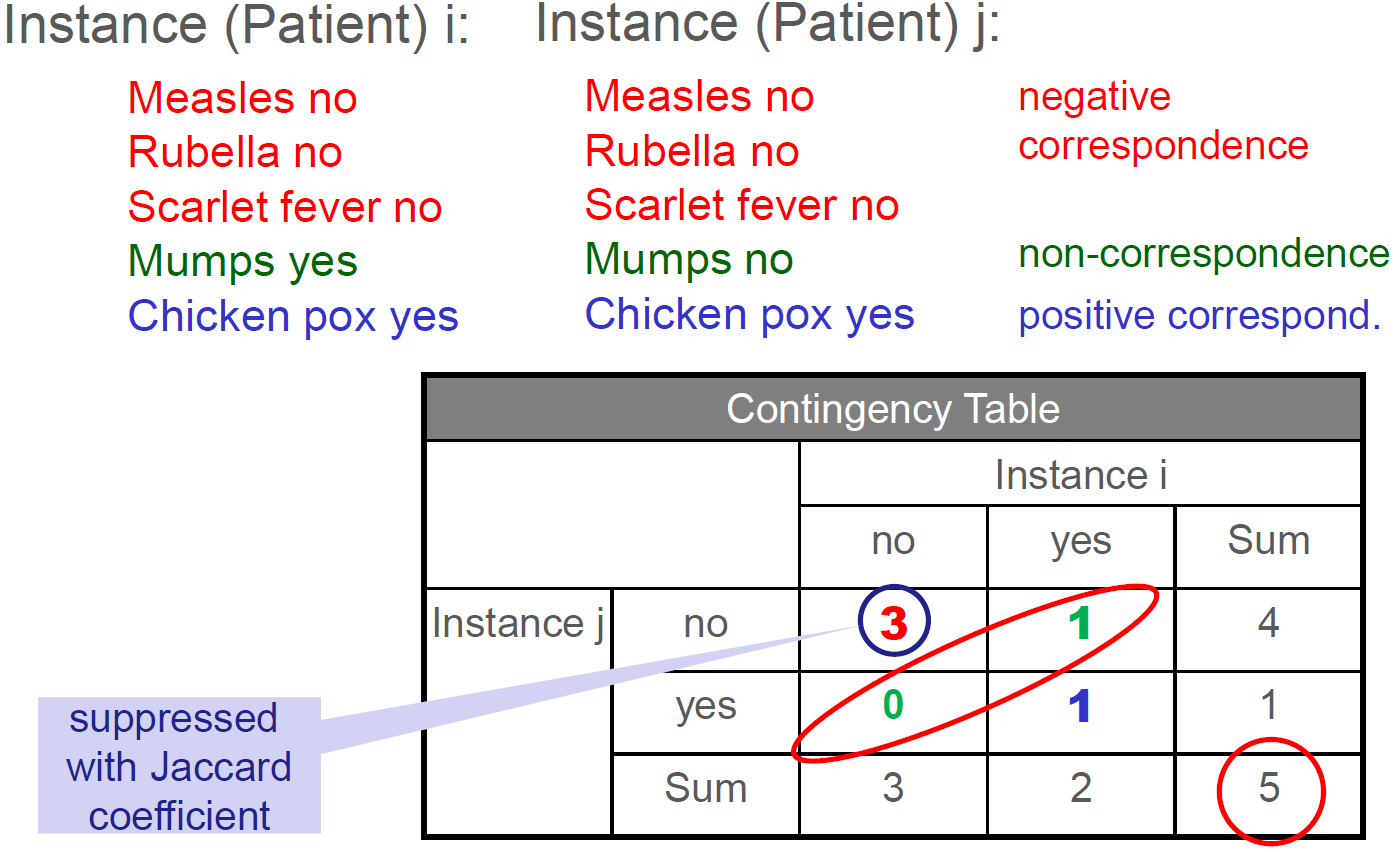
\includegraphics[width=.15\textwidth]{slides_images/clustering_binary_distance.png}
\end{center}

Jaccard coefficient: $d=\frac{0+1}{5-3} = \frac{1}{2}$

\end{breakbox}



\begin{breakbox}
\boxtitle{Distance of Nominal Data}

\begin{itemize}
	\item Nominal scale:
		\begin{itemize}
			\item red, yellow, blue, green, white
			\item food, health-care, toys, electronics
			\item $d=\frac{\# \text{attr} - \# \text{correspondences}}{\# \text{attr}}$			
		\end{itemize}
	\item Ordinal scale
		\begin{itemize}
			\item rank nominal data by some order, e.g. gold, silver, bronze
			\item calculate as usual, e.g. by Euclidean or Manhattan distance
		\end{itemize}
\end{itemize}

\end{breakbox}